\documentclass[]{elsarticle} %review=doublespace preprint=single 5p=2 column
%%% Begin My package additions %%%%%%%%%%%%%%%%%%%
\usepackage[hyphens]{url}

  \journal{Journal of Petroleum Science And Engineering} % Sets Journal name


\usepackage{lineno} % add
  \linenumbers % turns line numbering on
\providecommand{\tightlist}{%
  \setlength{\itemsep}{0pt}\setlength{\parskip}{0pt}}

\usepackage{graphicx}
\usepackage{booktabs} % book-quality tables
%%%%%%%%%%%%%%%% end my additions to header

\usepackage[T1]{fontenc}
\usepackage{lmodern}
\usepackage{amssymb,amsmath}
\usepackage{ifxetex,ifluatex}
\usepackage{fixltx2e} % provides \textsubscript
% use upquote if available, for straight quotes in verbatim environments
\IfFileExists{upquote.sty}{\usepackage{upquote}}{}
\ifnum 0\ifxetex 1\fi\ifluatex 1\fi=0 % if pdftex
  \usepackage[utf8]{inputenc}
\else % if luatex or xelatex
  \usepackage{fontspec}
  \ifxetex
    \usepackage{xltxtra,xunicode}
  \fi
  \defaultfontfeatures{Mapping=tex-text,Scale=MatchLowercase}
  \newcommand{\euro}{€}
\fi
% use microtype if available
\IfFileExists{microtype.sty}{\usepackage{microtype}}{}
\usepackage[margin=1in]{geometry}
\bibliographystyle{elsarticle-harv}
\usepackage{longtable}
\ifxetex
  \usepackage[setpagesize=false, % page size defined by xetex
              unicode=false, % unicode breaks when used with xetex
              xetex]{hyperref}
\else
  \usepackage[unicode=true]{hyperref}
\fi
\hypersetup{breaklinks=true,
            bookmarks=true,
            pdfauthor={},
            pdftitle={Bayesian Optimization : A New Sample Efficient Workflow for Reservoir Optimization under Uncertainty},
            colorlinks=false,
            urlcolor=blue,
            linkcolor=magenta,
            pdfborder={0 0 0}}
\urlstyle{same}  % don't use monospace font for urls

\setcounter{secnumdepth}{5}
% Pandoc toggle for numbering sections (defaults to be off)

% Pandoc citation processing
\newlength{\cslhangindent}
\setlength{\cslhangindent}{1.5em}
\newlength{\csllabelwidth}
\setlength{\csllabelwidth}{3em}
% for Pandoc 2.8 to 2.10.1
\newenvironment{cslreferences}%
  {}%
  {\par}
% For Pandoc 2.11+
\newenvironment{CSLReferences}[2] % #1 hanging-ident, #2 entry spacing
 {% don't indent paragraphs
  \setlength{\parindent}{0pt}
  % turn on hanging indent if param 1 is 1
  \ifodd #1 \everypar{\setlength{\hangindent}{\cslhangindent}}\ignorespaces\fi
  % set entry spacing
  \ifnum #2 > 0
  \setlength{\parskip}{#2\baselineskip}
  \fi
 }%
 {}
\usepackage{calc}
\newcommand{\CSLBlock}[1]{#1\hfill\break}
\newcommand{\CSLLeftMargin}[1]{\parbox[t]{\csllabelwidth}{#1}}
\newcommand{\CSLRightInline}[1]{\parbox[t]{\linewidth - \csllabelwidth}{#1}\break}
\newcommand{\CSLIndent}[1]{\hspace{\cslhangindent}#1}

% Pandoc header
\usepackage{setspace}
\usepackage{booktabs}
\usepackage{longtable}
\usepackage{array}
\usepackage{multirow}
\usepackage{wrapfig}
\usepackage{float}
\usepackage{colortbl}
\usepackage{pdflscape}
\usepackage{tabu}
\usepackage{threeparttable}
\usepackage{threeparttablex}
\usepackage[normalem]{ulem}
\usepackage{makecell}
\usepackage{xcolor}



\begin{document}
\begin{frontmatter}

  \title{Bayesian Optimization : A New Sample Efficient Workflow for Reservoir Optimization under Uncertainty}
    \author[a]{Peyman Kor\corref{1}}
  
    \author[a]{Aojie Hong}
  
    \author[a]{Reidar Brumer Bratvold}
  
      \address[a]{Energy Resources Department, University of Stavanger, Stavanger, Norway}
      \cortext[1]{Corresponding Author, peyman.kor@uis.no}
  
  \begin{abstract}
  \doublespacing An underlying challenge in well-control optimization during field development is that flow simulation of a 3D, full physics grid-based model is computationally prohibitive. In a robust optimization setting, where flow simulation has to be repeated over a hundred(s) of geological realizations, performing a proper optimization workflow becomes impractical in many real-world cases. In this work, to alleviate this computational burden, a new sample efficient optimization method is presented. In this context, sample efficiency means that the workflow needs a minimum number of forward model evaluations (flow-simulation in the case of reservoir optimization) while still being able to capture the global optimum of the objective function. Moreover, the workflow is appropriate for cases where precise analytical expression of the objective function is nonexistent. Such situations typically arise when the objective function is computed as the result of solving a large number of PDE(s), such as in reservoir-flow simulation. In this workflow, referred to as ``Bayesian Optimization'\,' the objective function for samples of decision variables is first computed using a proper design experiment. Then, a Gaussian Process (GP) is trained to mimic the surface of the objective function as surrogate model. While balancing the exploration-exploitation dilemma, a new decision variable is queried from the surrogate model and a flow simulation is run for this query point. Later, the output of the flow-simulation is assimilated back to the surrogate model which is updated given the new data point. This process continues sequentially until termination criteria are reached. To validate the workflow and get better insight about the details of optimization steps, we first optimize a 1D problem. Then, the workflow is implemented for a 3D synthetic reservoir model in order to perform robust optimization in a realistic field scenario. Finally, a comparison of the workflow with two other commonly used algorithms in the literature, namely Particle Swarm Intelligence (PSO) and Genetic Algorithm (GA) is performed. The comparison shows that the workflow presented here will reach same near-optimal solution achieved with GA and PSO, yet reduce computational time of the optimization 5X (times). We conclude that the method presented here significantly speeds up the optimization process leveraging a faster workflow for real-world 3D optimization tasks, potentially reducing CPU times by days or months, yet gives robust results that lead to a near-optimal solution. 
  \end{abstract}
   \begin{keyword} Optimization, Gaussian Process, Probabilistic Modeling, Bayesian\end{keyword}
 \end{frontmatter}

\newpage

\hypertarget{introduction}{%
\section{Introduction:}\label{introduction}}

\doublespacing

While developing a field, prediction of reservoir response to change in
the variable is an am important factor to have an efficient reservoir
management. The field of reservoir engineering is rich in the
development and application of full-physics numerical simulations for
forward modeling. However, the computational power needed to run such
numerical simulators most of the time is huge. Especially, the framework
of the Robust Optimization where uncertainty are considered through
multiple of geological realization (thousand or multi-thousand), the
practical applicability of such forward modeling is considerably
limited. To address this challenge, the proxy-modeling for reservoir
managemnet has emerged to reduce the cost of forward simulation. The
root of this field goes back to the work of the (Bruce, 1943) where the
analogy between flow of electricty in tthorugh te electrical device and
the response of the reservoir was constructed. (Albertoni and Lake, 2003) Proposed
the a Multivariate Linear Regression (MLR) to estimate the production
from the well, where it claimed that total production at each is linear
combination of injection rates with diffusitivity filter. Building on
the work of (Albertoni and Lake, 2003), (Yousef, 2006) proposed a new procedure to
quantify communication between wells, where for each injector/producer
pair, two coefficients, capacitance to quantify connectivity and time
constant to quantify the degree of fluid storage were considered.
(Sayarpour, 2008) used superposition in time to analytically solve the
numerical integration in CRM. (Zhao et al., 2015)(Zhao et al.~2015) articulated
that CRM models are not applicable when production rates change
significantly, mainly due to those models neglect to include intearction
of production-production and injector-injector pair well. Formulating
the model in the framework titled INSIM (interwell numerical simulation
model), it was used as efficient replacement to reservoir simulator when
history-matching phase rate data or water-cut data obtained during water
flooding operations.

Seperatley, in sake of utilization of recent advancemnet in the world of
Information technology, couple of reaserach has been don eon the
development of ``Surrogate Reservoir Models'' - (Mohaghegh and Guruswamy, 2006) proposed
the workflow for SRM model where Fuzzy Paatern Recognition (FPR)
technology was dimensionality reduction, in both static and dynamic
parameters of the reservir . Key Performance Indicator (KPI) was used to
select the most important variable.- (Sampaio, 2009) tried on use of
feed-forward neural networks as nonlinear proxies of reservoir response.
A few set of rock and fluid properties were considere a input (porosity,
permeability in ``x'' direction, permeability in ``y'' direction, and rock
compressibility) where in developing the neural network model, only one
hidden layer was used. flow proxy modeling to replace full simulation in
history matching, and built the proxy with a single hidden layer
artificial neural network (ANN). To predict the oil production from the
SAGD rocess, (Fedutenko et al.~2014) (Fedutenko et al., 2014)employed the RBF
Neural Network to predict the cumulative oil production over the time
horizon of production (10 years) .

\hypertarget{survey-of-suurgate--based-papers-in-onepetro-database}{%
\subsection{Survey of suurgate -based papers in onepetro database}\label{survey-of-suurgate--based-papers-in-onepetro-database}}

\newpage

\hypertarget{problem-statement}{%
\section{Problem Statement}\label{problem-statement}}

In general, an optimization task can be defined as a search process for the maximum output value of a ``well behaved''\footnote{In this context, it means the function is defined everywhere inside input domain, it is single-valued and continuous.} objective function \(f\). Can be defined as \(f: \chi \rightarrow \mathbb{R}\) where acceptable solutions \(\chi\), has a dimension of \(D\), \(\chi \subseteq \mathbb{R}^D\) :

\begin{equation}
\begin{aligned}
& \underset{x}{\text{maximize}}
& & f(x) \\
& \text{subject to}
& & x \subseteq \chi
\end{aligned}
\label{eq:globalopt}
\end{equation}

In Figure \ref{fig:optglobal} we can see some examples where the surface of \(f\) could be challenging to be optimized. The surfaces on the left side need careful attention to avoid getting stuck in local optima. Figures on the right side show presence of saddle area, where the gradient of function \(f\) is zero, in some cases in only one direction, possibly all directions. In this work, the focus is on the type of objective function \(f\), which is challenging to optimize because of the following three difficulties:

\begin{itemize}
\tightlist
\item
  \(f\) is explicitly unknown. This is a typical case in reservoir optimization problems where the Net Present Value (NPV) or Recovery Factor (RF) is computed through solving a vast number of partial differential equations through flow simulation. Thus, a precise analytical expression for the objective function is not available, avoiding the applicability of techniques that exploit the analytical expression of the objective function.
\item
  The surface of \(f\) is multi-modal. Meaning that \(f\) is non-convex in the domain of \(\chi\) , and the optimization algorithm must visit all local optima to find the ``global'' one.
\item
  Most importantly, forward evaluation of \(f\) is computationally expensive. This point will be discussed more in detail below.
\end{itemize}

\begin{figure}

{\centering 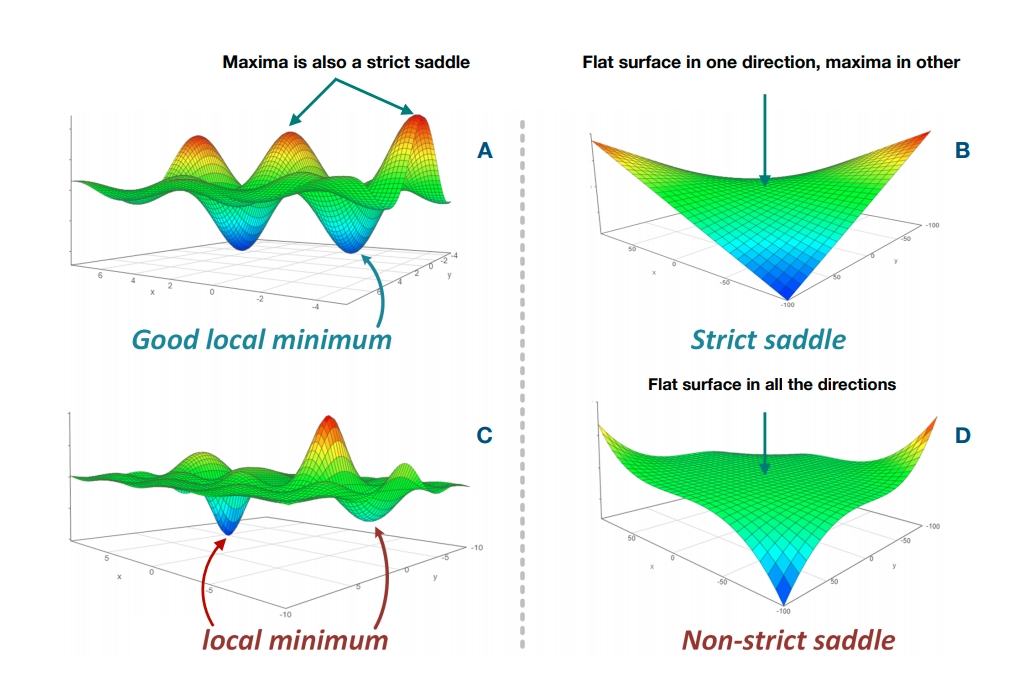
\includegraphics[width=0.7\linewidth]{img/globalopt} 

}

\caption{This plot may change, it does not show what exactly I want to say...}\label{fig:optglobal}
\end{figure}

In the examples of this paper, the goal is to maximize the subsurface-outcomes-based NPV (in USD). Thus, the primary objective function is also referred to as simply NPV in the rest of this paper. This objective function has been widely used in both well control and field development optimization studies. In a deterministic setting, the uncertainty in the geological parameters are disregarded and the optimization is performed based on a single geological model. Therefore, in the case of deterministic optimization, the objective function can be defined as:

\begin{equation}
J(\mathbf{u, G})= \sum_{k=1}^{K} \Bigg [\sum_{j=1}^{N_p}p_oq_{o,j,k}(\mathbf{u, G}) 
- \sum_{j=1}^{N_p}p_{wp}q_{wp,j,k}(\mathbf{u, G}) - 
\sum_{j=1}^{N_{wi}}p_{wi}q_{wi,j,k}(\mathbf{u, G}) \Bigg]\frac{\Delta t_k}{(1+b)^{\frac{t_k}{D}}}
\label{eq:npvdet}
\end{equation}

Where the first term in the double summation corresponds to the oil revenue; the second term is water-production cost and third term corresponds to the water-injection cost. Equation \eqref{eq:npvdet} is considered as objective function in the deterministic setting since only a single geological model is considered. The \(G\) in the Equation \eqref{eq:npvdet} is ``the geological model.'' The additional parameters in the Equation are as follows: \(K\) is the total number of timesteps; \(N_p\) is the total number of production wells subject to optimization; \(N_{wi}\) is the total number of water-injection wells subject to optimization; \(k\) is the timestep index; \(j\) is the well-number index; \(p_o\) is the revenue from oil production per unit volume (in USD/bbl); \(p_{wp}\) is the water-production cost per unit volume (in USD/bbl); \(p_{wi}\) is the water-injection cost per unit volume (in USD/bbl); \(q_o\) is the oil-production rate (in B/D); \(q_{wp}\) is the water-production rate (in B/D); \(q_{wi}\) is the water-injection rate (in B/D); \(\Delta t_k\) is the time interval for timestep \(k\) (in days); \(b\) is the discount rate (dimensionless); \(t_k\) is the cumulative time for discounting; and D is the reference time for discounting (\(D = 365\) days if b is expressed as a fraction per year and the cash flow is discounted daily). \(\mathbf{u}\) in Equation \eqref{eq:npvdet} is the control vector (i.e., a vector of control variables) defined as \(\mathbf{u} = [u_1, u_2, \cdots, u_N]^D\), where \(D\) is the number of control variables (dimension of optimization problem).

As mentioned above, Equation \eqref{eq:npvdet} lacks to capture the uncertainty in the geological model. In contrast, in a Robust Optimization (RO) setting, the objective is to optimize the expected value over all geological realizations (assumption here is decision maker is risk-neutral). The objective function for the RO setting then can be defined as: (in the case of equiprobable geological realization)

\begin{equation}
\overline{J}(\mathbf{u}) = \frac{\sum_{re=1}^{n_e} J(\mathbf{u,G_{re}})}{n_e}
\label{eq:npvopt}
\end{equation}

Where in Equation \eqref{eq:npvopt} contrary to Equation \eqref{eq:npvdet}, there is not one, rather \(n_e\) geological realizations, each of them written as \(G_{re}\). In this work, the objective is to optimize the Equation \eqref{eq:npvopt}, where it is simply EV value of NPV defined in \eqref{eq:npvdet} over all realizations.\\

It is well defined in the literature that optimizing Equation \eqref{eq:npvopt} is computationally prohibitive (de Brito and Durlofsky, 2021a; Hong et al., 2017a; Nwachukwu et al., 2018). Not only because thousand(s) of PDE have to be solved in the flow-simulation in order to compute the \(q_o, q_{wp}, q_{wi}\); the flow simulation must be enumerated over all realizations \(n_e\) to compute \(\overline{J}(u)\). Let's assume a simple case to illustrate the computational burden of this optimization problem. Assume that an E\&P enterprise is in the process of finding the bottom hole pressure of five injection wells and shut-in time of other five production wells, \(D=10\). The geology team of the enterprise comes up with 100 geological realizations of the model.(\(n_e=100\)). Now, if we suppose that the reservoir model is 3D with a moderate number of grid cells, it is not hard to imagine that flow-simulation of a fine grid model will take \textasciitilde1hr . Then, simply having 100 realizations means that each forward computation of \(\overline{J}(u)\) takes around \textasciitilde100 hr. Considering that the enterprise has to decide in 6 month period (in the best case, it can be interpreted as 6 months CPU running time), which means that a total number of available budget for running the forward model is\(\frac{6 \times 30 \times 24 }{100}= 43.2 \approx 50\) is around 50. The budget of only \(50\) forward model in ten-dimensional, non-linear, and non-convex optimization problem is relatively low. To put this in simple terms, if we say that each dimension of the control variable \(\mathbf{u}\), could be discretized into ten possible cases, then total available solutions for this optimization problem will be \(\text {Number of all possible solutions} = 10^{10}\). As it is clear, finding the best solution from a pool of ten billion possible solutions with only 50 shots is a pretty much hard undertaking.\\

The rest of this paper will be arguing that the Bayesian Optimization workflow has especial strength to deal with the three difficulties described above. Where the workflow needs to capture the optimum global point (area) while having a small forward evaluation budget.

\newpage

\hypertarget{bayesian-optimization-workflow}{%
\section{Bayesian Optimization Workflow}\label{bayesian-optimization-workflow}}

\hypertarget{overal-view}{%
\subsection{Overal View}\label{overal-view}}

Workflow to perform global optimization of multimodal black-box
functions:

\begin{itemize}
\item
  Step 1. Choose some initial design points and build a probabilistic
  model over the space of possible objective \(f\), this probabilistic
  model serves as prior.
\item
  Step 2. Combine prior and the likelihood to get a posterior of
  probabilistic model over the objective given some observations.
\item
  Step 3. Use the posterior to decide where to take the next
  evaluation \(\bf{x^*}\) according to some policy for decision making.
\item
  Step 4. Evaluet the \(f\) at \(\bf{x^*}\) and augment it to the initial
  data, in step 1.
\end{itemize}

Iterate between 2 and 4 until the evaluation budget is over. \#\# 3.1
Gaussian Process

\newpage

\hypertarget{step-1.-probalistic-model-as-prior}{%
\subsubsection{Step 1. Probalistic Model as Prior}\label{step-1.-probalistic-model-as-prior}}

\hypertarget{gaussian-process-gp}{%
\paragraph{Gaussian Process (GP)}\label{gaussian-process-gp}}

reference to the book (Murphy, 2022)

Key Assumption in (GP) is that: the function values at a set of \(M > 0\)
inputs, \(\bf{f} = [f(x_1), ...,f(x_M)]\), is jointly Gaussian, with mean
and Covariance

\begin{equation}
(\mu = m(x_1),...m(x_M))
\sum_{i,j}= \kappa(x_i,x_j)
\label{eq:mean_cov}
\end{equation}

and \(\kappa\) is a positive definite (Mercer) kernel. Suppose we have a
initial design points, set \(\mathcal{D} = {(x_n, y_n) : n = 1 : N}\),
where \(y_n = f(x_n)\) is the noise-free observation of the function
evaluated at \(x\).

Now we consider the case of predicting the outputs for new inputs that
may not be in \(\mathcal{D}\).

\begin{equation}
\bf{f_{*}} = [f(x_1),.., f(x_{N_{*}})]
\label{eq:pred_fun}
\end{equation}

By definition of the GP, the joint distribution \(p(\bf{f_X},f|X,X_*)\)
has the following form:

\begin{equation}
\begin{bmatrix}  {\bf {f}_X}  \\  {{\bf f}_*} \end{bmatrix} \sim\mathcal{N} \begin{pmatrix} (\begin{bmatrix}  {{\bf \mu}_X}  \\  {{\bf \mu}_*} \end{bmatrix}),\begin{bmatrix} {{\bf K}_{X,X}}  & {{\bf
K}_{X,*}}  \\  {{\bf \mathbf{K}^\intercal}_{X,*}} & {{\bf K}_{*,*} } \end{bmatrix}\end{pmatrix}
\label{eq:gp_model}
\end{equation}

\begin{equation}
  \begin{split}
\mu_X = [m(x_1),...,m(x_N)] \\ 
\mu^\ast = [m(x^\ast_1,...m(x^\ast_N))]
  \end{split}
\label{eq:mu_val}
\end{equation}

\begin{equation}
 \begin{split}
K_{X,X} = {\Large \kappa} (X,X; \theta) , \; \; \; \; \; \ size (N \times  N) \\
K_{X,\ast} = {\Large \kappa} (X,X_\ast; \theta), \; \; \; \; \; \ size (N \times N_*) \\
K_{\ast,\ast} = {\Large \kappa} (X_\ast, X_\ast; \theta), \; \; \; \; \; \ size(N_\ast \times N_\ast)
 \end{split}
\label{eq:cov_sign}
\end{equation}

\begin{tabu} to \linewidth {>{\raggedright}X>{\raggedright}X}
\toprule
Covariance Kernels & assumeing $h=||x-x'||$\\
\midrule
Gaussain & $\Large \kappa (x,x') =\sigma_f^2 exp(-\frac{h^2}{2\ell^2})$\\
Matern $\mu=\frac{5}{2}$ & $\Large \kappa (x,x') =\sigma_f^2(1 + \frac{\sqrt{5}|h|}{\ell}\frac{5h^2}{3\ell^2})exp(-\frac{ -\sqrt{5}|h|}{\ell})$\\
Matern $\mu=\frac{3}{2}$ & $\Large \kappa (x,x') =\sigma_f^2(1 + \frac{\sqrt{3}|h|}{\ell})exp(-\frac{-\sqrt{3}|h|}{\ell})$\\
Exponetial & $\Large \kappa (x,x') =\sigma_f^2 exp(-\frac{|h|}{\ell})$\\
Power-Exponetial & $\Large \kappa (x,x') =\sigma_f^2 exp(-(\frac{|h|}{\ell})^p)$\\
\bottomrule
\end{tabu}

\begin{equation}
{\Large \kappa} (x,x'; ;\theta) = (1 + \frac{\sqrt{5}|h|}{\theta} + \frac{5h^2}{3\theta^2})exp(-\frac{-\sqrt{5}|h|}{\theta}
\label{eq:pred_fun1}
\end{equation}

\hypertarget{covariance-kernel-parameter-estimation}{%
\paragraph{Covariance Kernel, Parameter estimation}\label{covariance-kernel-parameter-estimation}}

\begin{equation}
p(y|\bf{X,\theta}) = \int p(y|\bf{f,X})p(f|\bf{X,\theta})
\label{eq:lig_int}
\end{equation}

\begin{equation}
\text{log} p(y|\bf{X,\theta})=\mathcal{L}(\zeta,\sigma_f^2)=-\frac{1}{2}(y-\mu_X)^{\intercal}\mathbf{K}_{X,X}^{-1}(y-\mu_X)-\frac{1}{2}log|K_{X,X}|-\frac{n}{2}log(2\pi)
\label{eq:log_like}
\end{equation}

Where the dependence of the \(\bf{K}_{X,X}\) on \(\theta\) is implicit.The
gradient-based optimizer is performed in order to:

\begin{equation}
[\zeta^\ast, \sigma_f^{2\ast}]=argmax\mathcal{L}(\zeta,\sigma^2_f)
\label{eq:log_like_opt}
\end{equation}

However, since the objective \(\mathcal{L}\) is not convex, local minima
can be a problem, so we may need to use multiple restarts.

\hypertarget{step-2.-posterior-of-probabilistic-model}{%
\subsubsection{Step 2. Posterior of Probabilistic Model}\label{step-2.-posterior-of-probabilistic-model}}

\hypertarget{posterior-of-gaussain-process-conditioning-on-initial-data}{%
\paragraph{Posterior of Gaussain Process, (conditioning on initial data)}\label{posterior-of-gaussain-process-conditioning-on-initial-data}}

Here in \ref{fig:gaus-norm}

\begin{figure}

{\centering 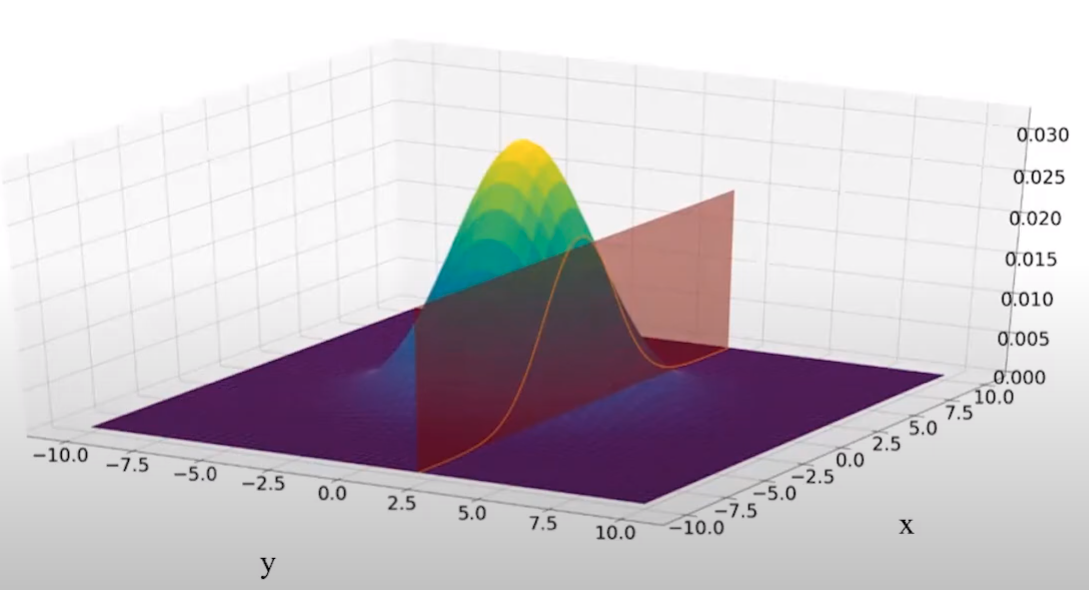
\includegraphics[width=400px,height=100px]{img/gaus_norm} 

}

\caption{proof of}\label{fig:gaus-norm}
\end{figure}

\begin{equation}
p(f_\ast|X_\ast,\mathcal{D}) = \mathcal{N}(f_\ast|{{\bf \mu}_\ast} , \scriptsize{\sum}_{\ast}\normalsize)
\label{eq:post_proba}
\end{equation}

\begin{equation}
  \begin{split}
{{\bf \mu}_\ast}=m(\bf X_\ast) +{\bf \mathbf{K}^\intercal}_{X,*}{\bf \mathbf{K}^{-1}}_{X,X}(f_X-m(X)) \\
\scriptsize{\sum}_{\ast}=\normalsize{\mathbf{K}_{\ast,\ast}-\mathbf{K}^\intercal_{X,\ast}\mathbf{K}_{X,X}^{-1}\mathbf{K}_{X,\ast}}
  \end{split}
\label{eq:post_mean_cov}
\end{equation}

\hypertarget{example-of-step.1-and-step.2}{%
\subsubsection{Example of Step.1 and Step.2}\label{example-of-step.1-and-step.2}}

Assume \(X=[0,3,5,6]\) and \(f_X=sin(X)\), giving \(\mathcal{D}=(X,f_X)\).
What is \(p(f_\ast|X_\ast,\mathcal{D})\)

\begin{figure}
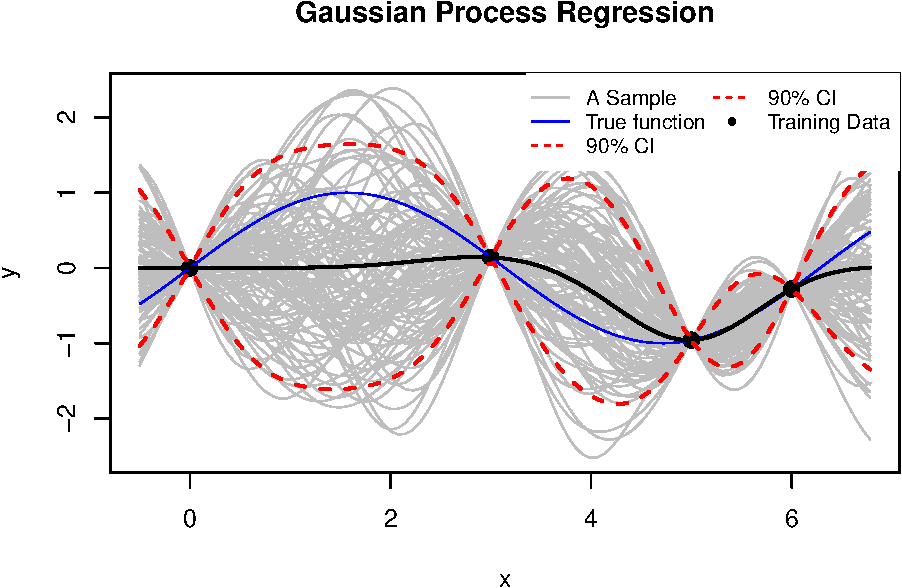
\includegraphics[width=1\linewidth]{0_Paper1_main_files/figure-latex/guass-1-1} \caption{Gaussin Process Regression conditioned on 4 points}\label{fig:guass-1}
\end{figure}

Now we sample the point \(X=1\), and add to \(\mathcal{D}\)

\begin{figure}

{\centering 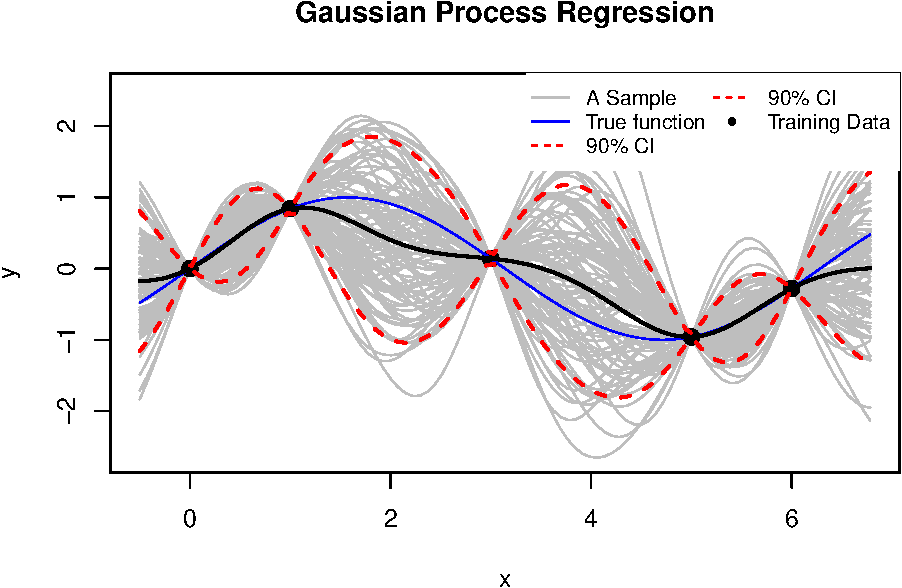
\includegraphics[width=1\linewidth,height=0.5\textheight]{0_Paper1_main_files/figure-latex/guass-2-1} 

}

\caption{Gaussin Process Regression conditioned on 5 points}\label{fig:guass-2}
\end{figure}

\hypertarget{step.3-deciding-on-next-bfxast-based-on-posterior}{%
\subsubsection{\texorpdfstring{Step.3 Deciding on next \(\bf{x}^\ast\) based on Posterior}{Step.3 Deciding on next \textbackslash bf\{x\}\^{}\textbackslash ast based on Posterior}}\label{step.3-deciding-on-next-bfxast-based-on-posterior}}

Posterior of the probalistic model quantify the uncertainty over the
space of the \(f\). The question is what is the next \(\bf{x}^\ast\) to be
sampled from the \emph{expensive function}?

Define an utility function to collect new data points satisfying some
optimality criterion: optimization as decision making.

There are a few of policies in the literature of Bayesopt, here the
\emph{Expected Improvement (EI)} policy will be used.

\hypertarget{expected-improvement-as-policy-for-decision-making}{%
\paragraph{Expected Improvement as Policy for Decision Making}\label{expected-improvement-as-policy-for-decision-making}}

In Expected Improvement (EI) policy choose the next query point as the
one which has the highest expected improvement over the space of the
\emph{expensive function}

\begin{equation}
utility(x;\theta,\mathcal{D})=\alpha_{EI}=\int_{y}^{}max(0,y-f)p(y|x;\theta,\mathcal{D})
\label{eq:uti_int}
\end{equation}

\[utility(x;\theta,\mathcal{D})=\alpha_{EI}=\int_{y}^{}max(0,y-f)p(y|x;\theta,\mathcal{D}) \,dy\]

However, we do not have access to the \emph{expensive function}, \(f\),
therefore we replace the \(f\) with the best available solution found so
far, \(y^+\)

\begin{equation}
utility(x;\theta,\mathcal{D})=\alpha_{EI}=\int_{y}^{}max(0,y-y^{\dagger})p(y|x;\theta,\mathcal{D}) \,dy
\label{eq:uti_int_2}
\end{equation}

\(y^{+}\) : The best solution found in the training dataset \(\mathcal{D}\)

The good news: The analytical form of the utility function is available
for the gaussian process

\begin{equation}
\gamma(\mathbf{x})=\frac{\mu(\mathbf{x;\theta,\mathcal{D}})-y^{\dagger}}{\sigma(\mathbf{x;\theta,\mathcal{D}})}
\label{eq:uti_int_gamma}
\end{equation}

\begin{equation}
utility(\mathbf{x};\theta,\mathcal{D})=\alpha_{EI}(x;\theta,\mathcal{D})=(\mu(x;\theta,\mathcal{D})-y^{\dagger})\Phi(\gamma(x)) + \sigma(x;\theta,\mathcal{D})\phi(\gamma(x))
\label{eq:uti_int2}
\end{equation}

Where \(\Phi(.)\) and \(\phi(.)\) are CDF and PDF of standard Gaussian
distribution.

It is too greedy in the context of the sequential decision making.
Therefore, an explorative term is added as explorative'' parameter
\(\epsilon\).

\begin{equation}
\gamma(\mathbf{x})=\frac{\mu(\mathbf{x;\theta,\mathcal{D}})-y^{\dagger}-\epsilon}{\sigma(\mathbf{x;\theta,\mathcal{D}})}
\label{eq:uti_greed_gamma}
\end{equation}

\begin{equation}
\alpha_{EI}(x;\theta,\mathcal{D})=(\mu(x;\theta,\mathcal{D})-y^{\dagger}-\epsilon)\Phi(\gamma(x)) + \sigma(x;\theta,\mathcal{D})\phi(\gamma(x))
\label{eq:uti_int_gred2}
\end{equation}

\hypertarget{bo-as-a-mapping-between-two-problems}{%
\paragraph{BO As a ``mapping'' between two problems}\label{bo-as-a-mapping-between-two-problems}}

BO is an strategy to transform the problem

\begin{equation}
u_M = \underset{u\in \text{constraints}}{\mathrm{argmax}}\overline{J}(u)
\label{eq:exp_eq}
\end{equation}

unsolvabale!

\begin{equation}
u^{next}=\underset{u\in \text{constraints}}{\mathrm{argmax}} \alpha_{EI}(u;\mathcal{D}_n, \theta^\ast)
\label{eq:exp-easy}
\end{equation}

solvabale!

\begin{itemize}
\tightlist
\item
  \(\alpha_{EI}(u)\) is inexpensive to evaluate.
\item
  The analytical expression for gradient of \(\alpha_{EI}(u)\) is
  available.
\item
  Still need to find \(u^{next}\), the multi-start BFGS is used for
  finding \(u^{next}\).
\end{itemize}

\newpage

\hypertarget{example-cases}{%
\section{Example Cases}\label{example-cases}}

\hypertarget{d-toy-problem}{%
\subsection{1-D toy Problem}\label{d-toy-problem}}

In this section, a 1-D toy problem is considered to illkuystrate the Bayes Optimization workflow dicussed in the previous section. The 1-D problem was selected sinnce it will help to visuluze all the steps of the workslow making easier explanation of the concepts. Though, it it can bee senn from the next section, the workflow can easily extened to to higer dimetional problem. The \emph{True function} to be optimized in this section has an analytical expression as, given the box constrains:

\begin{equation}
\begin{aligned}
& \underset{x}{\text{maximize}}
& & f(x) = 1-\frac{1}{2}(\frac{\sin (12x)}{1+x} + 2\cos(7x)x^5 + 0.7)  \\
& \text{subject to}
& & 0 \leq x \leq 1
\end{aligned}
\label{eq:1deq}
\end{equation}

Since the analytical expression of function available and being 1-D problem, the global optimum of the function had been found at the \(x_M = 3.90\). The plot of the function and the optimum point has been shown in the Figure \ref{fig:onedplot}

\begin{figure}

{\centering 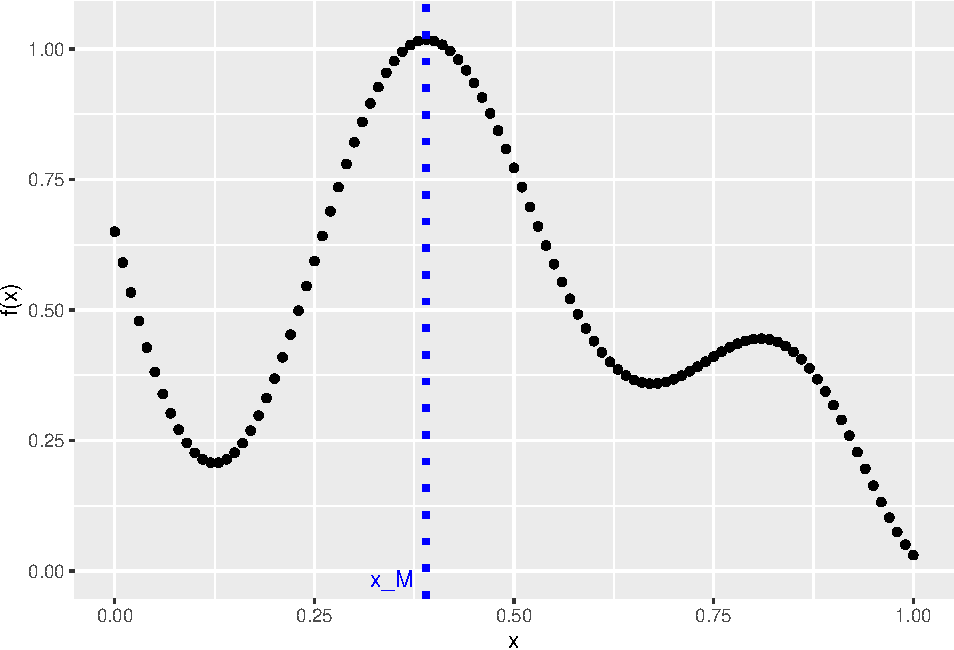
\includegraphics[width=0.9\linewidth]{0_Paper1_main_files/figure-latex/onedplot-1} 

}

\caption{Plot of 1-D equation with blue dash line representing the global optimum}\label{fig:onedplot}
\end{figure}

However, it is worth to mention that the analytical expression of objective function in many of real world problems are not avilable, what is avilable is a \emph{samples} from the objective function. Thefore, in the coming example a few samples are sequentiall drawn from the objective function to resemble the real case scenario. However, we know the global optimum of the objective function in hindsight, just in the case we want to copare the performace of Bayesian optimisation algorithem.

Thefore, as Figure \ref{fig:exampleshow}, the 5 sample points, \(x=[0.05,0.2,0.5,0.6,0.95]\) were selected as the initialization of the workflow. In the upper plot, blue lines represnets the samples from posterior of the gaussian model conditioned on the five sample points. The grey area represents the 95\% confidence interval while the red curve represents the mean value of the samples (blue lines). The first point to infer from the Figure \ref{fig:exampleshow} is there no uncertainty on the sample point. As shown, there is no grey zone on sample point since as was dicussed in the previous section, here we consider the ``noise-free'' observation. Also, worth to mention that we have wide more uncertainity (wider grey band) in the reas that are more distant from the observation, simply meaning we are less uncertain close to observation points. on the ``extrpolation,'' meaning in the ares outseide of the observation points, the probalistic model shows inetrsting behaviour. on those ``exterme'' area, the mean curve tend to move toward the mean of all observation points , here around 0, showing the model refelctes the mean-revervion behaviour when it comes extrpolation.

The lower part of Figure \ref{fig:exampleshow}, shows the plot of utility function at each x values. Worth to note that as the plot suggest, the utility(\(\alpha_{EI}\)) function will have the muti-modal structure, meaning in the optimization process multi-start gradient method will be helpful, in order to avoid stock in the local optima. In this work, as was explained in the preious section, the multi-start gradient method was used. The blue dotted line line shows the the \(x_{next}\) which is the point where the utility function, is maximum. Then this \(x_{next}\) is qured from the real function, and the the pair of \((x_{next}, f(x_{next}))\) is added to the intial data set, \(\mathcal{D}\). Going back to the lower figure at Figure \ref{fig:exampleshow}, the utility has two mode around point \(x=0.5\), say \(x_{0.5}^+\) and \(x_{0.5}^-\), however the point \(x_{0.5}^-\) is selected as the next query point. Readers can be rfereed to the upper plot and it is clear that there is more uncertainity around point \(x_{0.5}^-\) than \(x_{0.5}^+\) which given the form of utility function, that is understandable. The utility function always looking for the point that not only maximize the mean value, but also intereded in the points that has higher variannce, which is the case between two points \(x_{0.5}^+\) and \(x_{0.5}^-\).

\begin{figure}

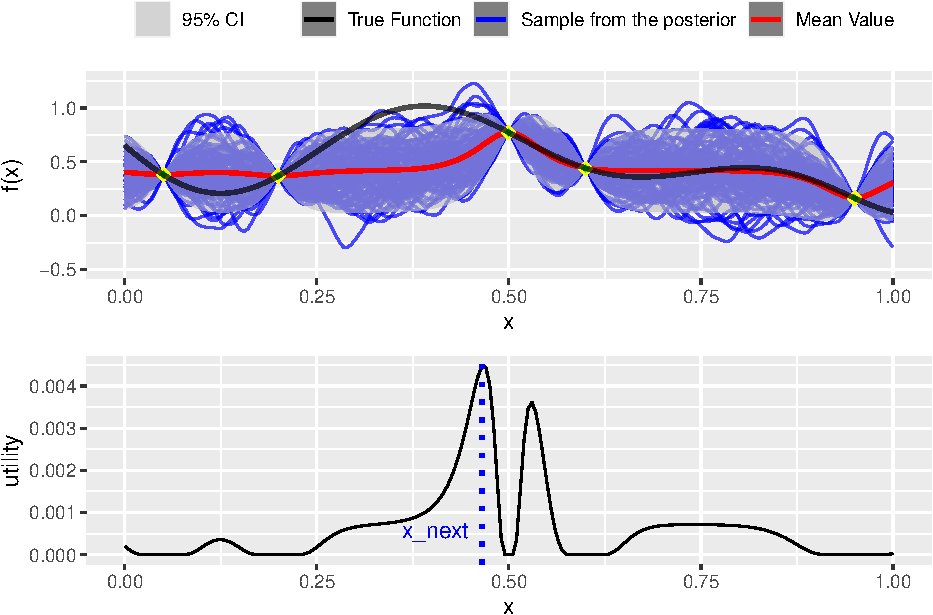
\includegraphics[width=1\linewidth,height=0.75\textheight]{0_Paper1_main_files/figure-latex/exampleshow-1} \hfill{}

\caption{Ite1 - Top: Gaussian posterior over the initial sample points; Lower: Utility function over the x values}\label{fig:exampleshow}
\end{figure}

Calling the Figure \ref{fig:exampleshow} as the iteration \# 1, now we can start sampling sequentially. In the Figure \ref{fig:allinone} another two iteration has been provided. Wher in each row, the plot on the left represents the posterior on the gaussian condistioning, the right show the utility function. Note that in the Figure \ref{fig:allinone} all axis labels and legned were not included, to have better visibity. (more info about each plot can ben found in \ref{fig:exampleshow}) . Interesting to see tat in this example case, at the irteration \#2, the workflow query the point \(x=0.385\) which presents the best point so far found through BayesOpt workflow. Thefiore, after just two iteration we are around \(\frac{x_{best}}{x_{M}}=\frac{0.385}{0.390}=98.7%
\) of the global optima. Although this is case for 1-D problem, it is clearly showing the stength of the workflow to approach the lglobal optima, in as few as possible iteration. In this case after iteration\#2, tyhe total number of tim,e that the real function has been quered is \(\text{size}(\mathcal{D}) + \text{size}(total iteration) = 5 + 2=7\) .

\begin{figure}

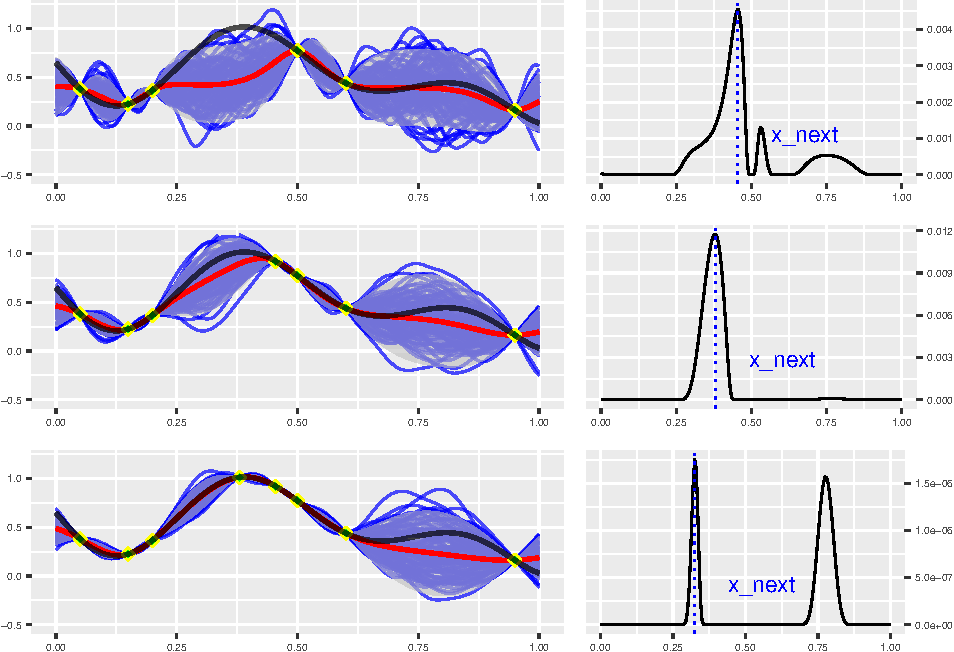
\includegraphics[width=0.9\linewidth,height=0.9\textheight]{0_Paper1_main_files/figure-latex/allinone-1} \hfill{}

\caption{Gaussian posterior of over the initial sample points}\label{fig:allinone}
\end{figure}

Before going to apply the same workflow at the field scale, the 1-D example presented here offer another useful feature of the Bayesian Optimisation. Looking at \ref{fig:allinone}, we can see that the maximum of utility function is at the iteration \# 3 in order of \(10^{-6}\) . That show that after optimization, eve best point to be queried in the next section has a very little utility. So can safely stop the process, since querying points to be sampled from the expensive function has a negligible potential to improve our search in optimization.

\newpage

\hypertarget{field-scale}{%
\subsection{Field Scale}\label{field-scale}}

\hypertarget{synthetic-3d-reservoir-model}{%
\subsubsection{Synthetic 3D Reservoir Model}\label{synthetic-3d-reservoir-model}}

In this section, the BayesOpt workflow is applied to the synthetic 3D reservoir model. The trough introduction of the model and gelogical describtion can be found in (Jansen et al., 2014) . Known as ``Egg Model'' it has a geology of channelized depositional system.

\begin{figure}

{\centering 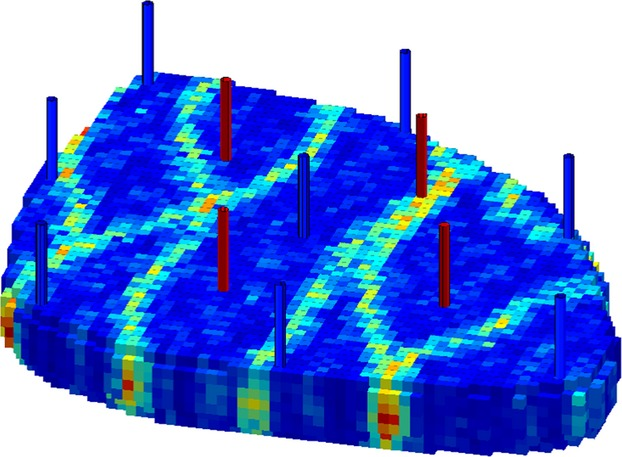
\includegraphics[width=300px]{img/egg_base} 

}

\caption{Well locations in Egg model, blue ones are injection, the red producers}\label{fig:eggbase}
\end{figure}

The 3D model has eight water injectors and four producers wells shown in Figure \ref{fig:eggbase}. The has a geological realizations of patterns of highly permeable channels which are described by 100 equi-probable geological realizations, three of which are illustrated in left side of Figure \ref{fig:combine}.(Hong et al., 2017b).

Relative permeabilities and the associated fractional flow curve of the model have shown in right side of Figure \ref{fig:combine} .All the wells are vertical and completed in all seven layers. Capillary pressure is ignored. The reservoir rock is assumed to be incompressible. The model has a life-cycle of 10 years. Here, the injection rate to be maiintaned over life-cycle of reservoir is going to be optimized. Thus, given eight injection wellls, the optimizatijon workflow has the eight dimnetions.However, the optimization in not unbounded, the water can be adjusted from 0 to 100 m3/day, making the box-constrain optimization. The injectors are operated with no pressure constraint, and the producers are under a minimal BHP of 395 bars without rate constraint.

\begin{figure}

{\centering 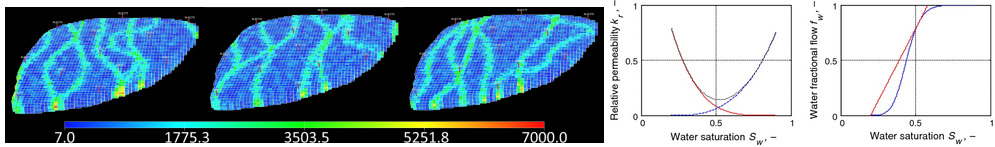
\includegraphics[width=1\linewidth]{img/combine} 

}

\caption{Left: Three geological realizations of the 3D model; Right: Rel perm and fractional flow curve}\label{fig:combine}
\end{figure}

\hypertarget{well-control-optimization}{%
\subsubsection{Well Control Optimization}\label{well-control-optimization}}

Reviewing the equation raised in the section 3, here the goal is robust optimization of the field , given geological realizations as follow:

\begin{equation}
\text{Objective Func(u)}= \overline{J}(u) = \frac{\sum_{i=1}^{n_e} J_r(u,G_i)}{n_e}  \label{eq:npvoptrep}
\end{equation}

Equation \eqref{eq:npvoptrep}

\(u\) is Injection rate for the each injection well, therefore the control vector, to be optimizaed in this case is defined as:

\begin{equation}
u=[u_{inj1},u_{inj2},u_{inj3},u_{inj4},u_{inj5},u_{inj6},u_{inj7},u_{inj8}]^{\intercal} 
\label{eq:cont-vec}
\end{equation}

As the \eqref{eq:npvoptrep} suggest, the \(\overline{J}(u)\) need some parameters to be defined. The oil price (\(P_o\)), water production cost (\(p_{wp}\)) and water injection cost (\(P_{wi}\)) in \(dollar/m^3\) has been provided in the Table \ref{tab:npvparam}. Also, in this work the cash flow is disconted daily and the discount factor is avilable in the \ref{tab:npvparam}. We would like to note that in this work due to avoid further computional burden in optimization process, 10 realizations of the egg model has been considered, therefore \(n_e=10\) in Equation \eqref{eq:npvoptrep}.

\begin{table}[H]

\caption{\label{tab:npvparam}Required Parameters needed for calculation of Expected NPV}
\centering
\begin{tabu} to \linewidth {>{\raggedright}X>{\raggedright}X>{\raggedright}X>{\raggedright}X}
\hline
Item & Pric & Items & Value\\
\hline
P\_o & 315 & b & 8\%\\
\hline
P\_wp & 47.5 & D & 365\\
\hline
P\_wi & 12.5 & n\_e & 10\\
\hline
\end{tabu}
\end{table}

\hypertarget{bayesopt-workflow}{%
\subsubsection{BayesOpt Workflow}\label{bayesopt-workflow}}

As it was discussed, the starting point of the BAyesOpt workflow is to randomly sample the initial data pairs \(\mathcal{D}\) which is used to build the Gaussian model of the response surface to the input variables. In this work, forty samples fom the Latin hyper cube sampling (LHS) method were drawn. The LHS is prefred in this work to Monte Carlo since it provides the stratifcation of the CDF of each variable, leading to better coverage of the input variable space. The Figure \ref{fig:lhssampling} show the results of the \(\overline{J}(u)\) for each sample from LHS. Also, The maximum \(\overline{J}(u)\) found from sampling has been shown with blue line. Setting the specific seed number (since LHS is in itself is random process), we get the max \(NPV\) aciehved here was \(35.65 \$MM\). Looking at Figure \ref{fig:lhssampling} it is worth to mention that random sampling like the LHS is not helpful to consistently approach the global optimum point, and there is a need for efficient workflow to find the optimum point while using the a few as possible sampling from real function.

\begin{figure}

{\centering 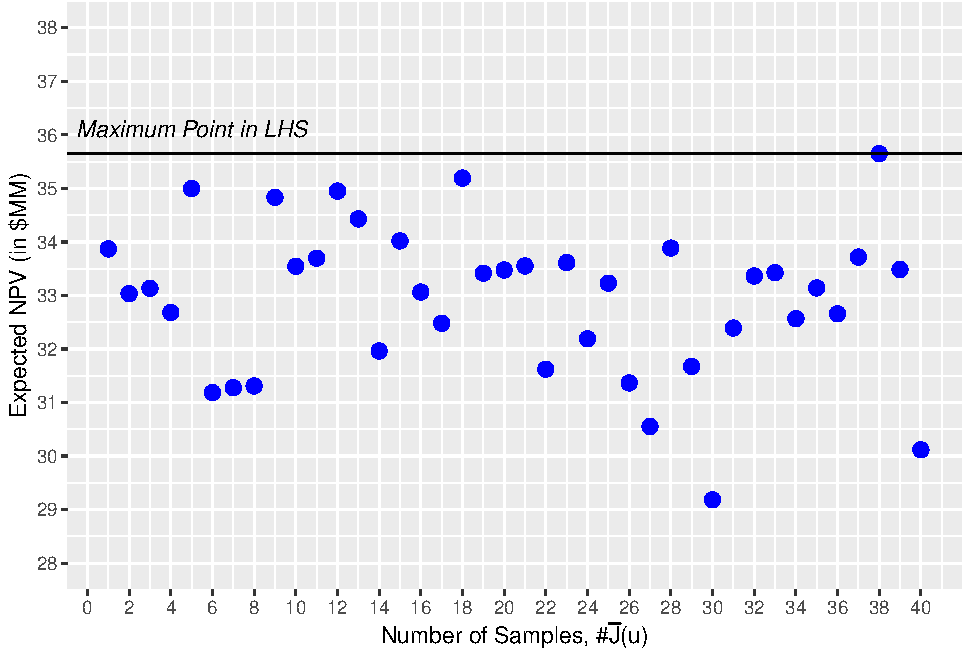
\includegraphics[width=468px]{0_Paper1_main_files/figure-latex/lhssampling-1} 

}

\caption{Expected NPV as result of forty sampling from LHS}\label{fig:lhssampling}
\end{figure}

Having the initial data found through LHS, we can build the probalistic model of the reposnse surface and sequentially sample from the \emph{expensive-to-evaluate} function. Unfortunately, win this section we can not plot the posterior of the probalistic model, condition on the above forty LHS samples, due being the space is eight-dimetional, and hard to visulize. The Figure \ref{fig:lhsbayesop} shows the expected NPV found after ten sequential sampling resulted from the BayesOpt workflow. Readers are refreed to this point that in the figure, not all red points are increasing and some points are lower than previous points. The reason for this behaviour is the nature of BayesOpt algorith. We can suggest that in the points that has lower expected NPV from the previous, we may reached the lower optimum point, but those points helped us to decrease the uncertainity, which is helpful for the further sampling. We can see that after just ten evaluation of the expenside function (here it means finding the expected NPv from running 10 geological realization using flow simulation) we reach the new record Expeted NPV of \(max \overline{J}(u)=36.85\)\(\$MM\).

\begin{figure}

{\centering 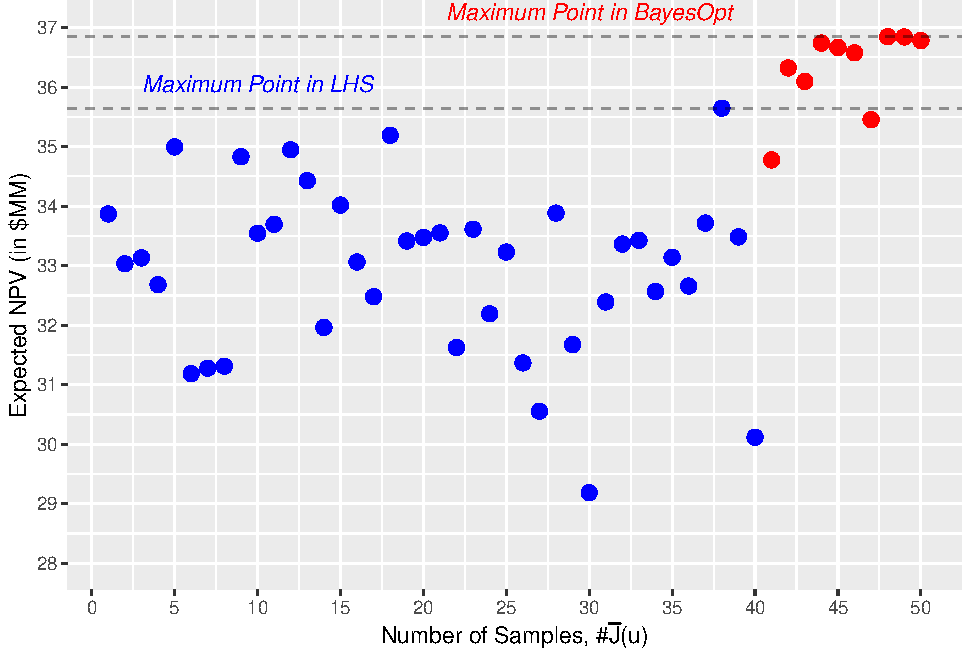
\includegraphics[width=468px]{0_Paper1_main_files/figure-latex/lhsbayesop-1} 

}

\caption{Blue points represnts the sample from LHS, red points represents the samples from the BayesOpt Workflow}\label{fig:lhsbayesop}
\end{figure}

Now, as we explained in the 1-D section, the plot of the utility at each iteration could provide some useful information about the optimization process. The Figure \ref{fig:utilitycurve} plots the \(\alpha_{EI}^*(\mathcal{D}, \theta^*)\) (Equation \eqref{eq:exp-easy} )versus the ten iteration in this work. In fact the notaion \(\alpha_{EI}^*\) means the optimum of the \(\alpha_{EI}(u;\mathcal{D},\theta^*)\) after running multi-start (1000)- L-BFGS-B on all \(u\) values. Now, we can see that in the figure the \(\alpha_{EI}^*\) is decreasing going toward the zero. It can be inferred from this trend that, we are going out of the \emph{good} \(u\) values to be sampled from the expensive function, can be intepreted that we are in the vicinity of global optima, if we see after several iteration still \(\alpha_{EI}^*\) is less than \(10^-6\).

\begin{figure}

{\centering 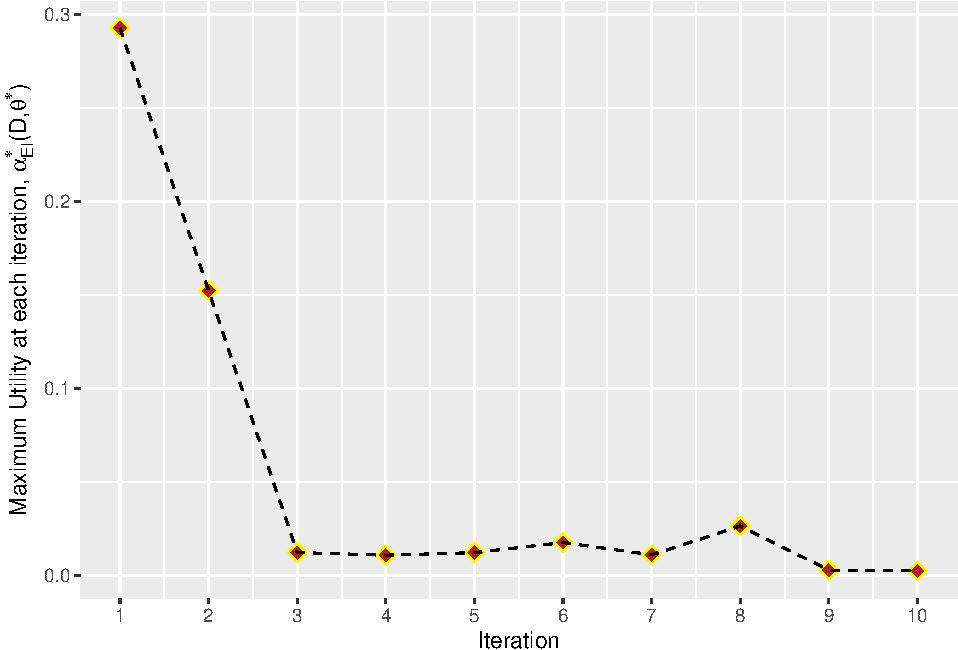
\includegraphics[width=468px]{0_Paper1_main_files/figure-latex/utilitycurve-1} 

}

\caption{Maximum utility at each iteration, after running L-BFGS-B to find the u with max utility, $\alpha_{EI}^*$}\label{fig:utilitycurve}
\end{figure}

Given that the BayesOpt inherintely has stochasric natrae ( from this perspective that having thje diffrenet initialization in LHS sampling will affect the final solution), in this section BayesOpt is repeated with diffret initilization. Ideally, this repeation shouwl be conducted 100 or 1000 times, to get better overview of the convergence of the algorithm given diffrent initilization. Though, because of the computional burden, in this work only three repeations were performed. optimization Repeat the Optimization, three times, in different initial design points. Figure \ref{fig:difinit} shows results of three repeations. At each repeation (top, middle, bottom), the blue dots come from diffrente seed numbers and they are diffrente. Then, gicen that initialization \(\mathcal{D}\), sequential sampling from the expenive function is perfomred, shown in the red points. Like previous case, in these repeations, 40 samples drawn from LHS algortihem, the 10 were taken thorigh BAyesOpt lagorith, totaling 50 samples. At each row of the Figure \ref{fig:difinit}, two horizontal lines show the maximum point \(\overline{NPV}\) in both random sampling phase (LHS) and BayesOpt phase. As it can be noted from the Figure \ref{fig:difinit}, at each repeation, the BayesOpt will improve the solution with small sample evaluation of the \(\overline{J}(u)\). Thefore, improvemnet following the BayesOpt phase indepned of the initial design, yet the bigger question is whether given different initial design, the algorithm converge the vicinity of global optima. What is refered here is that if having different initilaization will lead completely different final solution, that hints that the algorithm has a ``local'' search, in conrast, if the solutions leads to one specif close \(u^*\), that reprsents that algorithm have a ``global'' view on the surface of the objective function. In the case of ``global'' optimization having diferent initilizatin should lead to simular final solution, since the algorithm will not get stuck in local optimum points, close to initilalized data. This is common practice in the gradient-based optimization where the algorithm is powerfull in local optimization and in order to avoid stuck in local exterme points, ``multi-start'' runs are performed in order to search the global point in the objective function.

\begin{figure}

{\centering 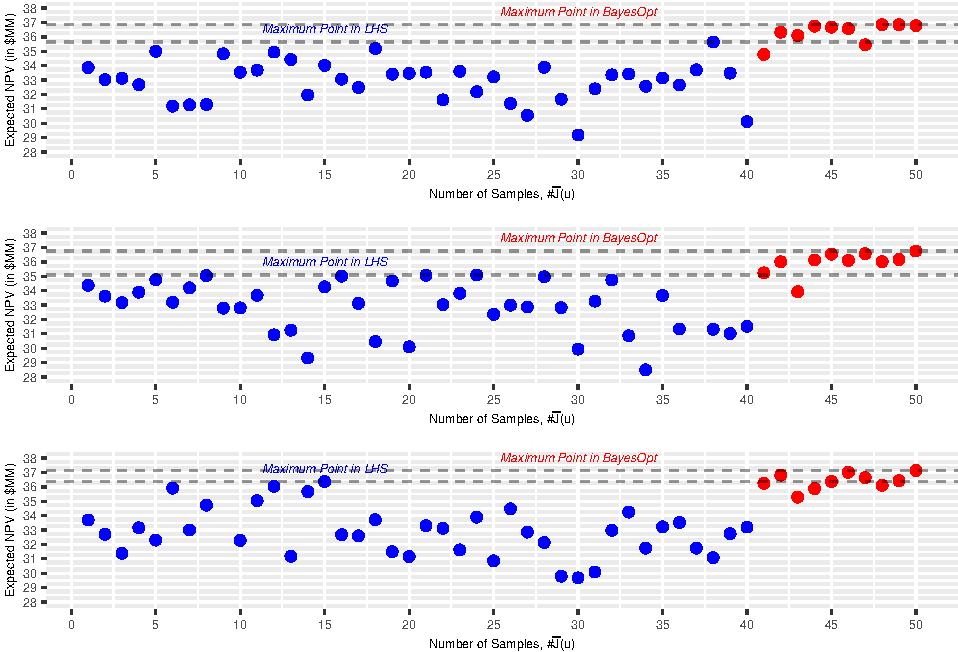
\includegraphics[width=0.9\linewidth,height=0.9\textheight]{0_Paper1_main_files/figure-latex/difinit-1} 

}

\caption{BayesOpt workflow applied to Syntetic 3D model, in three different initialization}\label{fig:difinit}
\end{figure}

To further continue thiss dicussion on the effect of initialization on the final solution, the \(u^*\) value for each repeatation has been show on the left side of Figure \ref{fig:diffu}. Where the \(u^*\) is the vector of 8 dimention, each value shows the optimum injection rate for the 10 years life cycle of the field, in \(m^3/D\). We woul like to note that the y axis was plotted from the range of 5 to 100. The reason for this is to show that in this optimization problem, injection of each wells can take any number between 5\(m^3/D\) to 100 \(m^3/D\), and the y axis shows the full extend of the value optimum zation worlkflow can reach. Visually, looking at the left plot at Figure \ref{fig:diffu}, we can see that the final solution of three repeations at each weels, does not differ significantly from each other . With small exception of (injection \#2), it seems all the final solutions converges to the same solution. This feature that can be loosly said as ``robustness'' of optimization workflow to initial design is very helpfu, from this sense that we do not neeed to resetart the optimization with different initilaization, since they all will converges to the similar solution. From this perspective, authours can infere that BayesOpt workflow can be considered as ``global'' optimization method, as it shows the workflow avoids stuck in local exterme pointsor saddle regions. The plot on the left side of Figure \ref{fig:diffu} shows that mean injection rate (mean of three repeations) and erro bar at each injection wells. The bottom of error bar in this plot shows the \(mean-sd\) and top of bar is \(mean + sd\) . As we can see that we do not see significant variation in the final solution in each repeations, also the plots recoomnds that in the case of repeating the optimization with more than three times (like 10 or 100), it can lead to lower variation in final solution.

\begin{figure}

{\centering 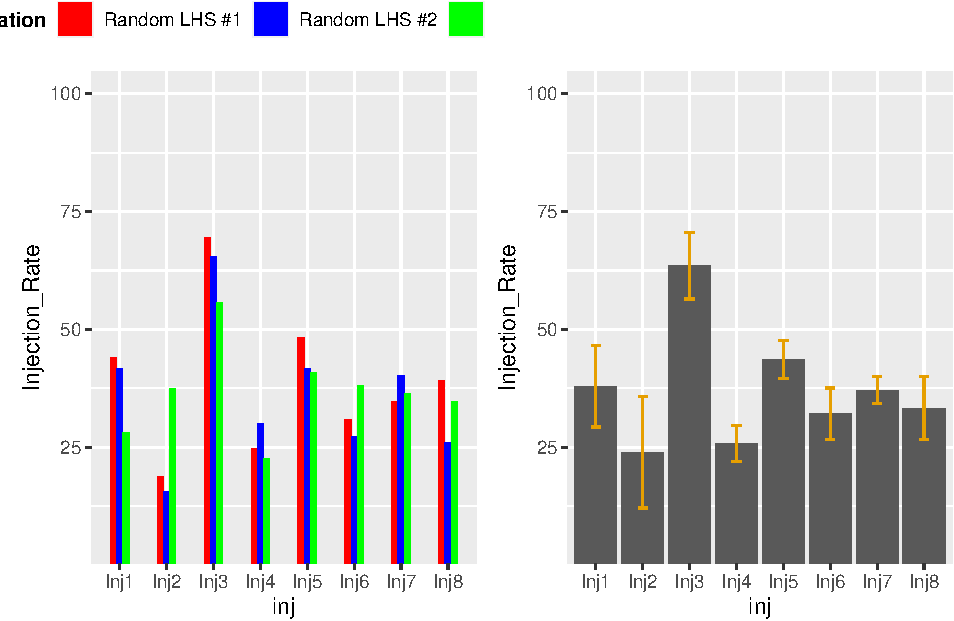
\includegraphics[width=0.9\linewidth]{0_Paper1_main_files/figure-latex/diffu-1} 

}

\caption{Left: final solution of optimization algorithm in three different initialization, Right: Mean and error bar of each injection rate at each injection wells}\label{fig:diffu}
\end{figure}

\newpage

\newpage

\hypertarget{bayesopt-performnace-versus-other-alternatives}{%
\section{BayesOpt performnace versus other alternatives}\label{bayesopt-performnace-versus-other-alternatives}}

In this section the aim is to compare the performance of the Bayeopt workflow with other availbale optimization alghorithm commonly used for reservoir optimization under uncertainity. The literature of field development optimzation enjoys wide varieties of the workflow and algorithm applied to field development. Broadly speaking those can be divided into two categories adjoint-gradient and derivative-free. Adjoint methods, such as those described in (Forouzanfar and Reynolds, 2014; Li and Jafarpour, 2012; Volkov and Bellout, 2018) can provide computational advantage in terms of efficiency. They are, however, local methods, and it is known that broad (global) searches can be advantageous in field development optimization methods.(de Brito and Durlofsky, 2021b) - Thefefore, in this work two well-know Derivative-free optimization (DFO) methods, extensively used rservoir optimization, named Genetic Algorithem (GA) (Chai et al., 2021; Holland, 1992a) and Particle Swarm Optimization (PSO) (Eberhart and Kennedy, 1995a; Jesmani et al., 2016) have been considered. In this section we provide a brief overview of each methods, but interested readers are reffered to the original papers.(Eberhart and Kennedy, 1995b; Holland, 1992b)

PSO is a global stochastic search technique that operates based on analogies to the behaviors of swarms/flocks of living organisms. Originally developed by Eberhart and Kennedy, Considering a swarm with \(P\) particles, there is a position vector \(X_{i}^{t}=(x_{i1},x_{i2}, x_{i3},x_{in})^T\) and a velocity vector \(V^t_i=(v_{i1},v_{i2},v_{i3},v_{in})^T\) at a \(t\) iteration for each one of the \(i\) particle that composes it. These vectors are updated through the dimension \(j\) according to the following equations:

\begin{equation}
V^{t+1}_{ij} = \omega V^{t}_{ij} + c_{1}r_{1}^{t}(pbest_{ij}-X_{ij}^t) + c_2r_2^t(gbest_j-X_{ij}^{t})
\label{eq:pso}
\end{equation}

where \(i=1,2,..., P\) and \(j =1,2,...,n\). Equation \eqref{eq:pso} explains that there are three different contributions to a particle's movement in an iteration. In the first term, the parameter \(\omega\) is the inertia weight constant. In the second term, The parameter \(c1\) is a positive constant and it is an individual-cognition parameter, and it weighs the importance of particle's own previous experiences. The other parameter second term is \(r_1^t\), and this is a random value parameter with {[}0,1{]} range. The third term is the social learning one. Because of it, all particles in the swarm are able to share the information of the best point achieved regardless of which particle had found it, for example, \(gbestj\). Its format is just like the second term, the one regarding the individual learning. Thus, the difference \((gbest_j - X^t_{ij})\) acts as an attraction for the particles to the best point until found at some t iteration. Similarly, \(c_2\) is a social learning parameter, and it weighs the importance of the global learning of the swarm. And \(r_2\) plays exactly the same role as \(r_1\). Where Equation \eqref{eq:psoup} updates the particle's positions. (Almeida and Leite, 2019)

\begin{equation}
X_{ij}^{t+1} = X_{ij}^{t} + V_{ij}^{t+1}
\label{eq:psoup}
\end{equation}

BayesOpt VS. with other Global Optimization Algorithms

Fixed Reservoir Simulation Budget (N=50)

\begin{center}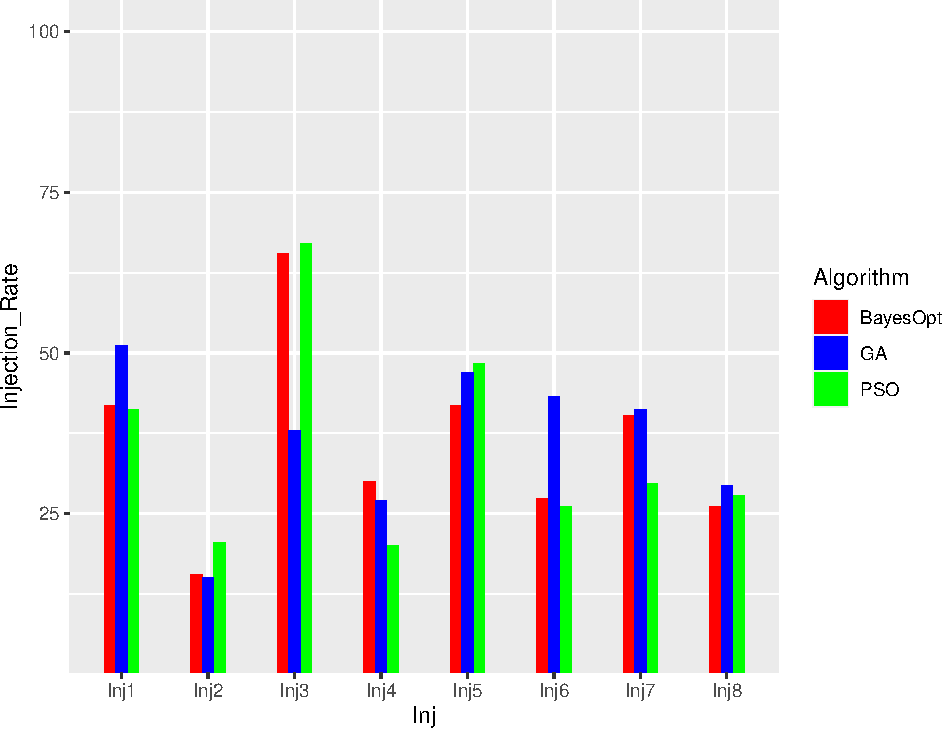
\includegraphics[width=468px]{0_Paper1_main_files/figure-latex/unnamed-chunk-11-1} \end{center}

BO: Reservoir Simulation Budget (N=50), GA, PSO: Reservoir Simulation Budget (N=250)

\begin{center}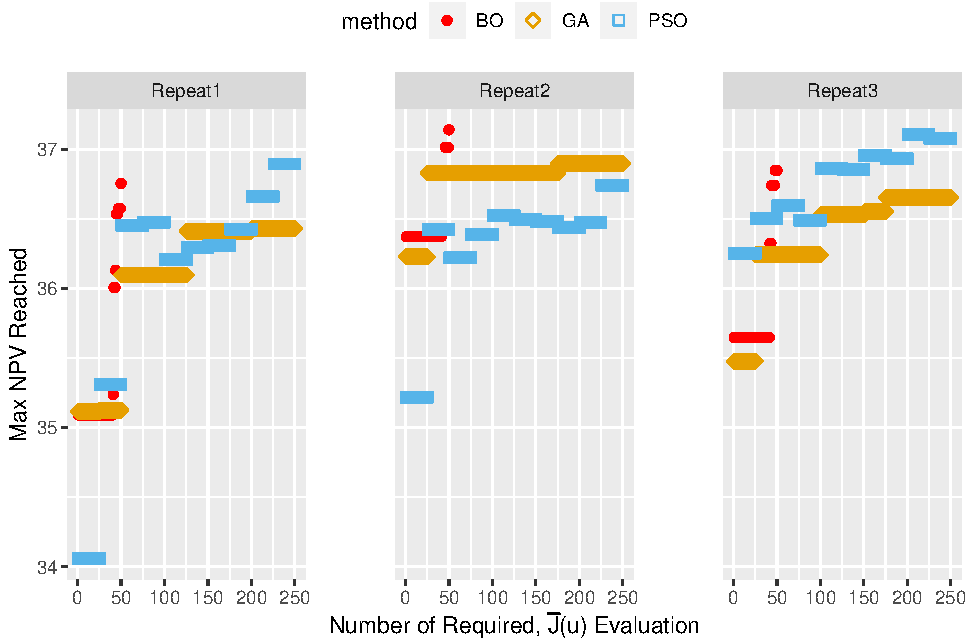
\includegraphics[width=468px]{0_Paper1_main_files/figure-latex/unnamed-chunk-12-1} \end{center}

BayesOpt VS. with other Global Optimization Algorithms

Table Summarizing Comparison of BayesOpt, PSO, GA

Comparing the Final Solution \(u\) of the Opt algorithms\ldots(the Median Replication was used)

\begin{center}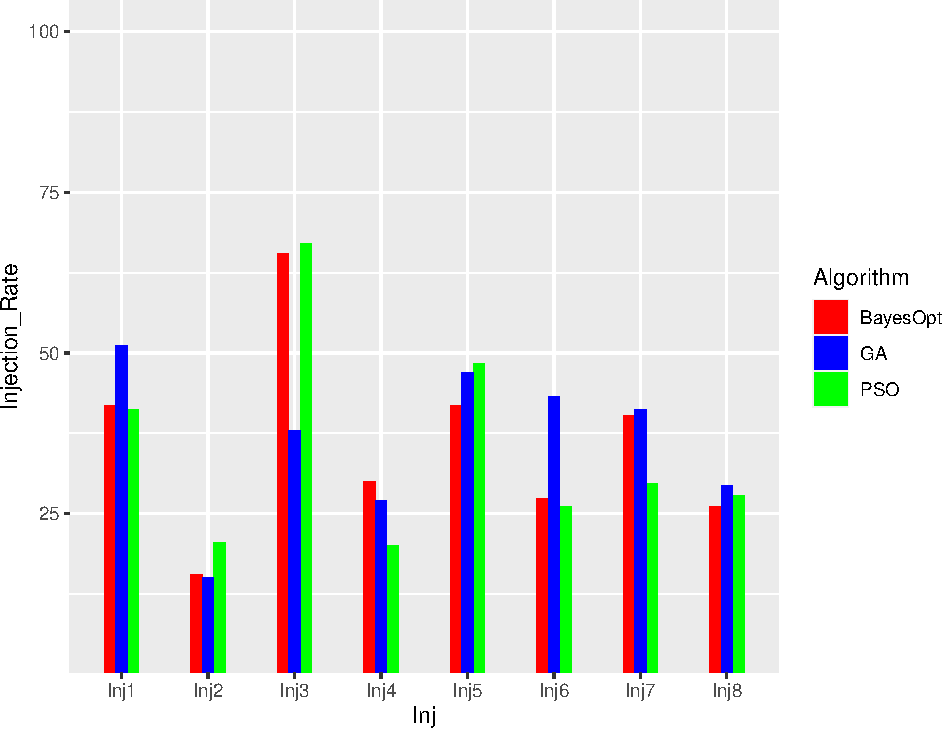
\includegraphics[width=468px]{0_Paper1_main_files/figure-latex/unnamed-chunk-14-1} \end{center}

\newpage

\hypertarget{conclusing-remarks}{%
\section{Conclusing Remarks}\label{conclusing-remarks}}

\newpage

\hypertarget{acknowledgements}{%
\section{Acknowledgements}\label{acknowledgements}}

This work received support from the Research Council of Norway and the companies AkerBP, Wintershall--DEA, Vår Energy, Petrobras, Equinor, Lundin, and Neptune Energy, through the Petromaks--2 DIGIRES project (280473) (http://digires.no). We acknowledge the access to Eclipse licenses granted by Schlumberger.

\newpage

\hypertarget{references}{%
\section*{References}\label{references}}
\addcontentsline{toc}{section}{References}

\hypertarget{refs}{}
\begin{CSLReferences}{1}{0}
\leavevmode\vadjust pre{\hypertarget{ref-albertoni2003}{}}%
Albertoni, A., Lake, L.W., 2003. Inferring Interwell Connectivity Only From Well-Rate Fluctuations in Waterfloods. SPE Reservoir Evaluation \& Engineering 6, 6--16. doi:\href{https://doi.org/10.2118/83381-PA}{10.2118/83381-PA}

\leavevmode\vadjust pre{\hypertarget{ref-almeida2019}{}}%
Almeida, B.S.G. de, Leite, V.C., 2019. Particle Swarm Optimization: A Powerful Technique for Solving Engineering Problems. IntechOpen.

\leavevmode\vadjust pre{\hypertarget{ref-bruce1943}{}}%
Bruce, W.A., 1943. An Electrical Device for Analyzing Oil-reservoir Behavior. Transactions of the AIME 151, 112--124. doi:\href{https://doi.org/10.2118/943112-G}{10.2118/943112-G}

\leavevmode\vadjust pre{\hypertarget{ref-chai2021}{}}%
Chai, Z., Nwachukwu, A., Zagayevskiy, Y., Amini, S., Madasu, S., 2021. An integrated closed-loop solution to assisted history matching and field optimization with machine learning techniques. Journal of Petroleum Science and Engineering 198, 108204. doi:\href{https://doi.org/10.1016/j.petrol.2020.108204}{10.1016/j.petrol.2020.108204}

\leavevmode\vadjust pre{\hypertarget{ref-debrito2021}{}}%
de Brito, D.U., Durlofsky, L.J., 2021b. Field development optimization using a sequence of surrogate treatments. Computational Geosciences 25, 35--65. doi:\href{https://doi.org/10.1007/s10596-020-09985-y}{10.1007/s10596-020-09985-y}

\leavevmode\vadjust pre{\hypertarget{ref-debrito2021a}{}}%
de Brito, D.U., Durlofsky, L.J., 2021a. Field development optimization using a sequence of surrogate treatments. Computational Geosciences 25, 35--65. doi:\href{https://doi.org/10.1007/s10596-020-09985-y}{10.1007/s10596-020-09985-y}

\leavevmode\vadjust pre{\hypertarget{ref-eberhart1995}{}}%
Eberhart, R., Kennedy, J., 1995a. A new optimizer using particle swarm theory. Ieee, pp. 39--43.

\leavevmode\vadjust pre{\hypertarget{ref-eberhart1995a}{}}%
Eberhart, R., Kennedy, J., 1995b. A new optimizer using particle swarm theory. Ieee, pp. 39--43.

\leavevmode\vadjust pre{\hypertarget{ref-fedutenko2014}{}}%
Fedutenko, E., Yang, C., Card, C., Nghiem, L.X., 2014. SPE Heavy Oil Conference-Canada. SPE, Calgary, Alberta, Canada, p. D021S008R001. doi:\href{https://doi.org/10.2118/170085-MS}{10.2118/170085-MS}

\leavevmode\vadjust pre{\hypertarget{ref-forouzanfar2014}{}}%
Forouzanfar, F., Reynolds, A.C., 2014. Joint optimization of number of wells, well locations and controls using a gradient-based algorithm. Chemical Engineering Research and Design 92, 1315--1328.

\leavevmode\vadjust pre{\hypertarget{ref-holland1992b}{}}%
Holland, J.H., 1992a. Adaptation in natural and artificial systems: An introductory analysis with applications to biology, control, and artificial intelligence. MIT press.

\leavevmode\vadjust pre{\hypertarget{ref-holland1992c}{}}%
Holland, J.H., 1992b. Adaptation in natural and artificial systems: An introductory analysis with applications to biology, control, and artificial intelligence. MIT press.

\leavevmode\vadjust pre{\hypertarget{ref-hong2017cg}{}}%
Hong, A.J., Bratvold, R.B., Nævdal, G., 2017b. Robust production optimization with capacitance-resistance model as precursor. Computational Geosciences 21, 1423--1442. doi:\href{https://doi.org/10.1007/s10596-017-9666-8}{10.1007/s10596-017-9666-8}

\leavevmode\vadjust pre{\hypertarget{ref-hong2017a}{}}%
Hong, A.J., Bratvold, R.B., Nævdal, G., 2017a. Robust production optimization with capacitance-resistance model as precursor. Computational Geosciences 21, 1423--1442. doi:\href{https://doi.org/10.1007/s10596-017-9666-8}{10.1007/s10596-017-9666-8}

\leavevmode\vadjust pre{\hypertarget{ref-jansen2014}{}}%
Jansen, J.D., Fonseca, R.M., Kahrobaei, S., Siraj, M.M., Essen, G.M.V., Hof, P.M.J.V. den, 2014. The egg model {\textendash} a geological ensemble for reservoir simulation. Geoscience Data Journal 1, 192--195. doi:\href{https://doi.org/10.1002/gdj3.21}{10.1002/gdj3.21}

\leavevmode\vadjust pre{\hypertarget{ref-jesmani2016}{}}%
Jesmani, M., Bellout, M.C., Hanea, R., Foss, B., 2016. Well placement optimization subject to realistic field development constraints. Computational Geosciences 20, 1185--1209. doi:\href{https://doi.org/10.1007/s10596-016-9584-1}{10.1007/s10596-016-9584-1}

\leavevmode\vadjust pre{\hypertarget{ref-li2012}{}}%
Li, L., Jafarpour, B., 2012. A variable-control well placement optimization for improved reservoir development. Computational Geosciences 16, 871--889.

\leavevmode\vadjust pre{\hypertarget{ref-mohaghegh2006}{}}%
Mohaghegh, S.D., Guruswamy, S., 2006. Development of Surrogate Reservoir Models (SRM) for Fast-Track Analysis of Complex Reservoirs. San Antonio, Texas, U.S.A, p. 9.

\leavevmode\vadjust pre{\hypertarget{ref-murphy2022}{}}%
Murphy, K.P., 2022. Probabilistic machine learning: An introduction. MIT Press.

\leavevmode\vadjust pre{\hypertarget{ref-nwachukwu2018}{}}%
Nwachukwu, A., Jeong, H., Sun, A., Pyrcz, M., Lake, L.W., 2018. SPE Improved Oil Recovery Conference. OnePetro. doi:\href{https://doi.org/10.2118/190239-MS}{10.2118/190239-MS}

\leavevmode\vadjust pre{\hypertarget{ref-sampaio2009}{}}%
Sampaio, T.P., 2009. An Application of Feed Forward Neural Network as Nonlinear Proxies for the Use During the History Matching Phase 11.

\leavevmode\vadjust pre{\hypertarget{ref-sayarpour2008}{}}%
Sayarpour, M., 2008. Development and application of capacitance-resistive models to water/CO? floods (PhD thesis).

\leavevmode\vadjust pre{\hypertarget{ref-volkov2018}{}}%
Volkov, O., Bellout, M.C., 2018. Gradient-based constrained well placement optimization. Journal of Petroleum Science and Engineering 171, 1052--1066.

\leavevmode\vadjust pre{\hypertarget{ref-yousef2006}{}}%
Yousef, A.A., 2006. A Capacitance Model To Infer Interwell Connectivity From Production- and Injection-Rate Fluctuations 17.

\leavevmode\vadjust pre{\hypertarget{ref-zhao2015}{}}%
Zhao, H., Kang, Z., Zhang, X., Sun, H., Cao, L., Reynolds, A.C., 2015. SPE Reservoir Simulation Symposium. Society of Petroleum Engineers, Houston, Texas, USA. doi:\href{https://doi.org/10.2118/173213-MS}{10.2118/173213-MS}

\end{CSLReferences}


\end{document}
